\chapter{El proceso de ETL}
\label{chap:etl}
Buscando que el modelo pueda ser reentrenado periódicamente, diseñamos un proceso de ETL que obtiene los datos, los limpia y aplica transformaciones para modificar variables o crear variables nuevas. Este proceso se lleva a cabo de forma orquestada en un servidor EC2 de AWS, haciendo peticiones a una base de datos RDS alojada en un servidor externo. En la medida de lo posible, el código está optimizado para efectuar la mayor cantidad de operaciones posibles con los recursos del RDS en lugar de utilizar los recursos del servidor de orquestación.
\par
\noindent
El proceso de ETL tiene tres fases: primero, los datos se extraen de la base de datos cruda y se efectúan procesos sencillos de limpieza de variables y corrección de tipos. Se procede a hacer una recodificación de variables para mayor comparabilidad entre poblaciones, y finalmente se crean variables nuevas a partir de los datos limpios.
\section*{Limpieza}
El proceso de limpieza se orquesta como una tarea de Luigi que ejecuta un código de R con el nombre de la tabla como parámetro de entrada, así como datos que permiten la conexión a la base de datos. Utilizamos R porque sus herramientas de manipulación de datos facilitan una gran cantidad de operaciones y permiten escribir código extremadamente legible. Este código de R, a su vez, busca en un directorio predeterminado códigos de limpieza específicos para la tabla en cuestión, que pueden estar escritos en R o en SQL. La limpieza se lleva a cabo como una operación remota hacia la base de datos, y el resultado queda guardado en una tabla temporal.
\par
\noindent
A pesar de que tenemos códigos de limpieza específicos para cada tabla, se diseñó un estándar para facilitar las llamadas a cada programa, sobre todo en el caso de los códigos escritos en R. Así, cada código de limpieza ejecuta una sola función, llamada \textit{make\_clean}.
\section*{Recodificación}
Para garantizar mayor comparabilidad y facilitar el entrenamiento, construimos un proceso de recodificación, que a través de uniones entre tablas permite homologar los nombres y valores de las variables que describen la misma característica de conjuntos de datos distintos. Así, se toma el resultado de la limpieza y se buscan las variables para las cuales hay códigos nuevos. Se hacen uniones entre la tabla limpia y la tabla auxiliar de códigos (mostrada en la figura abajo), explotando las capacidades de evaluación no estándar que permite R como se puede apreciar en el código expuesto en el anexo.
\par
\noindent
Para reducir la carga de procesamiento de la base de datos, cada recodificación se guarda de forma temporal y se usa ese resultado para hacer la siguiente recodificación. Una vez recodificada toda la tabla, se escribe el resultado temporal al esquema limpio.
\begin{figure}[h]
    \caption{Estructura general de la tabla auxiliar de recodificación. Cada fila representa un valor específico de la variable indicada por la columna ''variable\_inicial'', que forma parte de la tabla cruda especificada en la columna ''tabla''.}
    \centering
    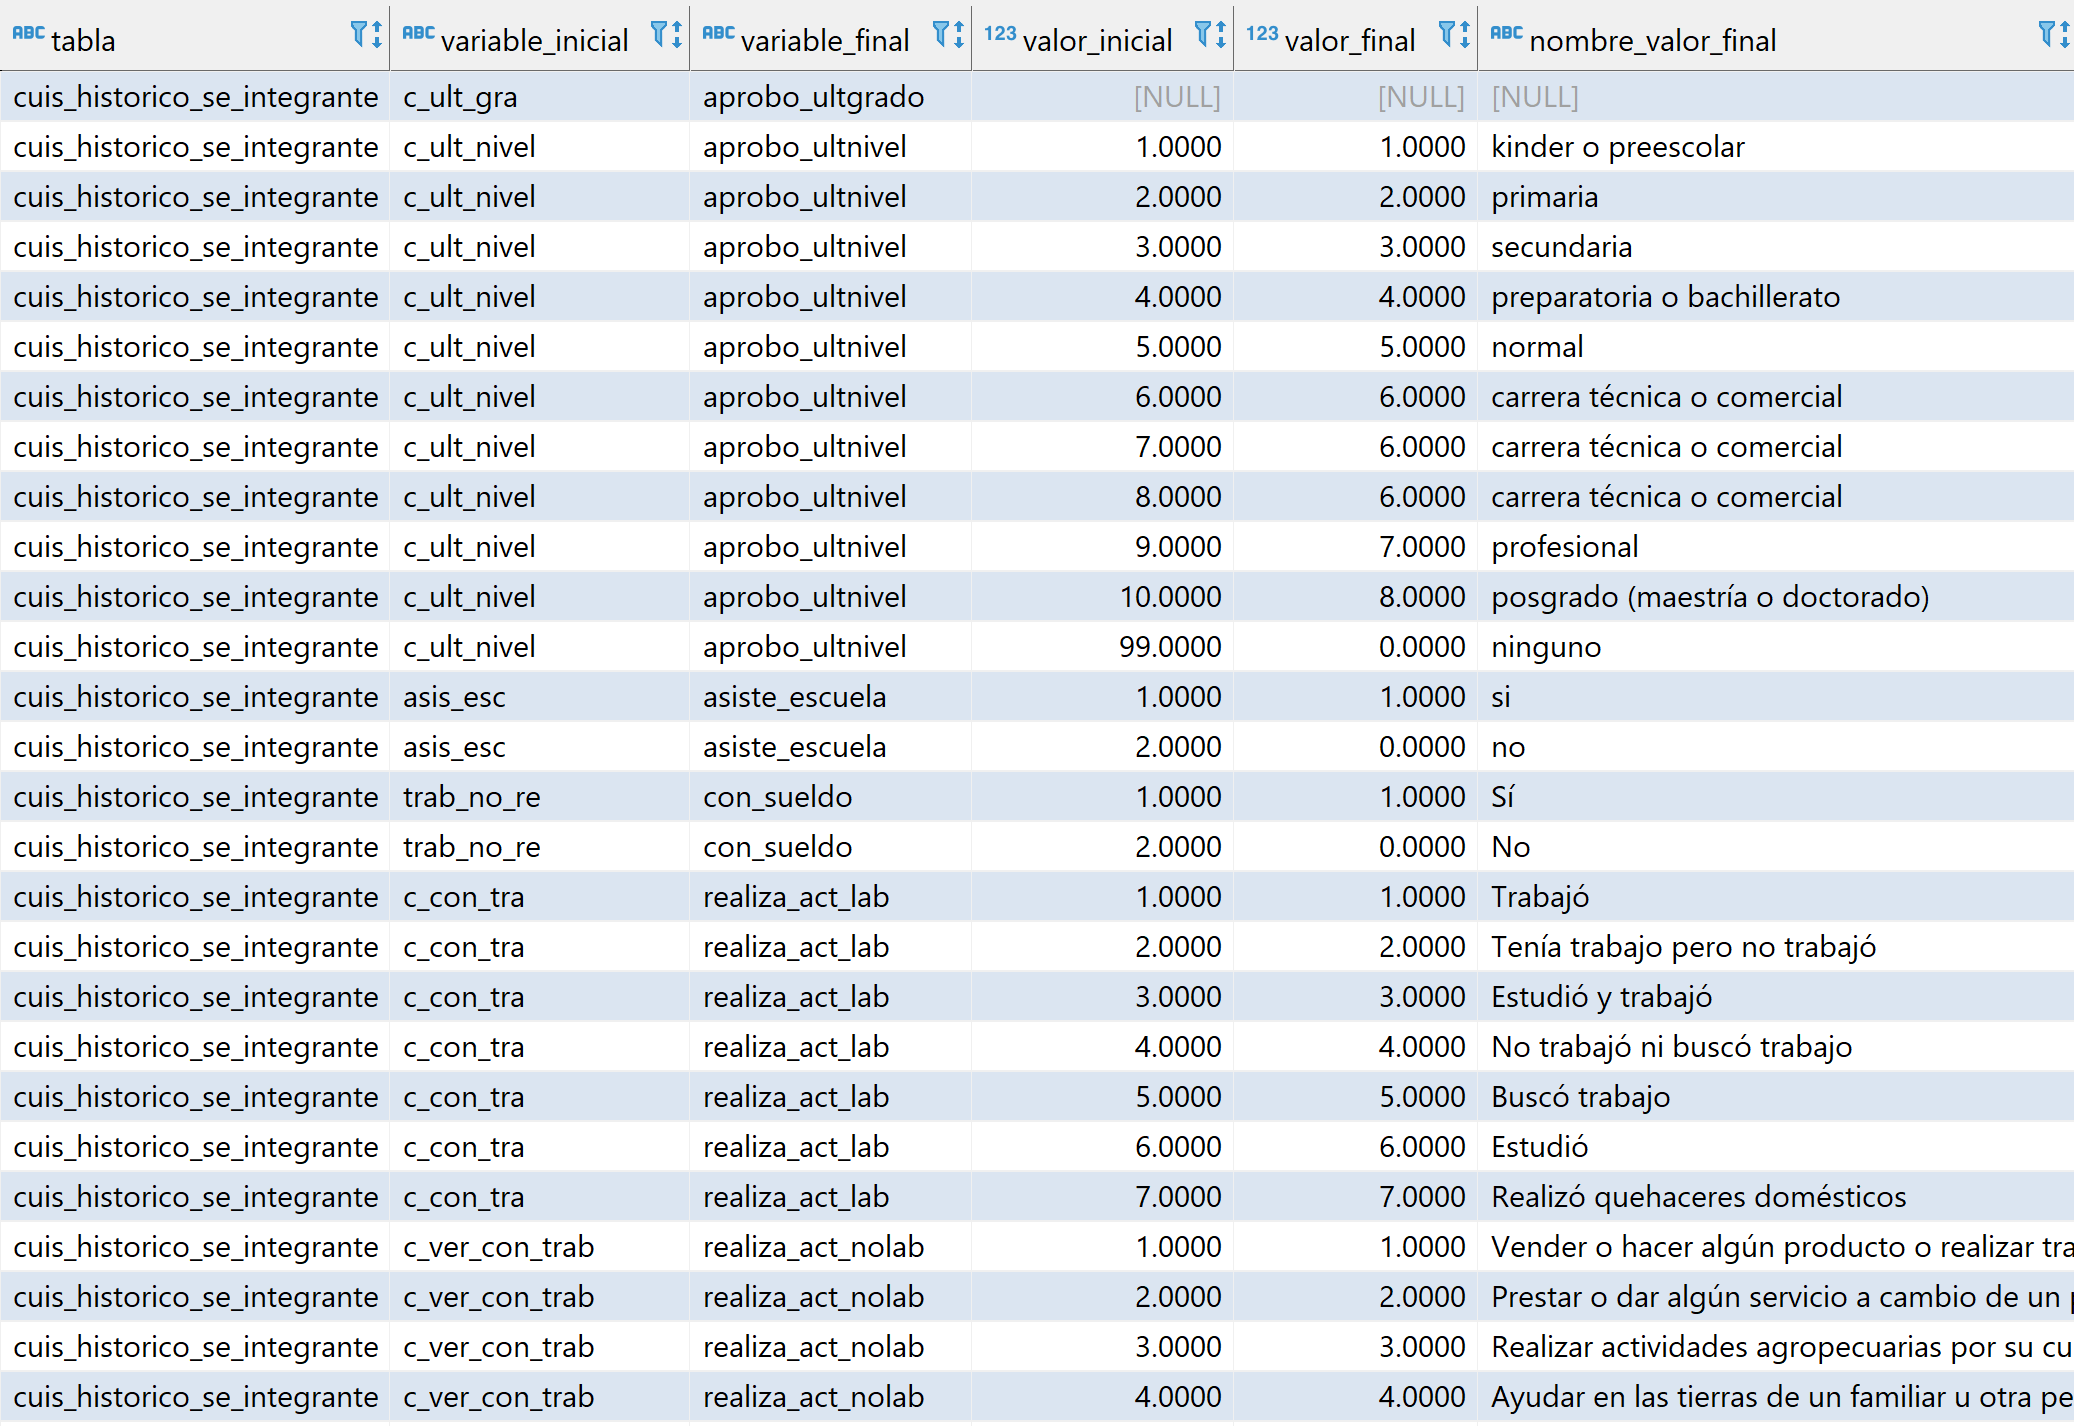
\includegraphics[width=8cm]{recode.png}
\end{figure}
\section*{Creación de variables nuevas}
Una vez escrita la tabla limpia a su esquema correspondiente, se utilizan esos datos para la creación de variables nuevas. La creación de variables nuevas está definida en un flujo de datos separado al proceso de ETL, buscando facilitar la idempotencia de las transformaciones. Así, las tablas de variables nuevas se escriben en un schema distinto en la base de datos, al que llamamos \textit{features}. Este flujo de datos se lleva a través del mismo orquestador, utilizando un archivo auxiliar de tipo \textit{YAML} para definir las dependencias que tienen estas tablas de nuevas variables. Estas dependencias pueden ser tablas limpias, tablas de resultados de modelos u otras tablas del mismo esquema de \textit{features}. El orquestador principal, llamado \textit{Features Pipeline}, recibe como parámetro el nombre de la tabla de variables nuevas, y busca en un archivo separado de configuración las fechas para las que tiene que correr el proceso de creación de variables nuevas. Cuando obtiene esa lista de fechas, busca cuáles son las dependencias de esa tabla en particular en el archivo \textit{YAML} y verifica que estén completas.
\par
\noindent
Una vez verificado que el proceso de limpieza esté completo para todas las dependencias, se busca un código de R específico para esa tabla de \textit{features}. Buscamos crear las mismas variables para muchas fuentes de datos distintas -en este caso, tenemos CUIS, ENCASEH y ENIGH- por lo que estandarizamos el proceso para auxiliarse de un archivo \textit{YAML} que define todos los conjuntos de variables a crear, así como datos adicionales como variables de agrupamiento o tipo de operación a realizar. Este archivo, así como las funciones auxiliares para procesarlo, se utiliza para todas las fuentes de datos para las que se vayan a crear esas variables. De esta forma, tenemos prácticamente el mismo proceso aplicado a tres fuentes de datos distintas.
\par
\noindent
En el archivo \textit{YAML} que contiene las variables nuevas, definimos abstracciones que nos permiten efectuar el mismo tipo de operación cuantas veces sea necesario, utilizando la misma función auxiliar. Tenemos tres tipos de funciones auxiliares, que toman una cadena de texto y la analizan sintácticamente para ejecutar las operaciones ahí indicadas, y se diferencian en la forma de analizar esa cadena de texto:
\begin{itemize}
    \item \textbf{\textit{get\_dummy}}: Analiza la cadena de texto como una condición lógica, verificando su valor de verdad. Regresa una variable dicotómica que responde al valor de verdad encontrado.
    \item \textbf{\textit{get\_func}}: Analiza la cadena de texto literalmente, como una instrucción válida a realizar en R. Un ejemplo de esto puede ser una multiplicación entre dos variables.
    \item \textbf{\textit{get\_cases}}: Analiza la cadena de texto como un conjunto de casos a considerar, de modo que la cadena de texto en este tipo de función tendría la forma $condicion \rightarrow resultado$, donde $condicion$ es una condición lógica, y $resultado$ es el valor que toma la variable en caso de verificarse que la condición es verdadera.
\end{itemize}
Tomamos entonces el nombre de la nueva variable, la cadena de texto a evaluar, el tipo de función que la va a evaluar y posiblemente un conjunto de datos auxiliares, como si existen variables de agrupamiento o filtros a aplicar antes de hacer la transformación. De esta forma, basta con seleccionar el conjunto de variables que se van a crear a partir del archivo \textit{YAML} y se puede entonces utilizar un conjunto muy sucinto y legible de funciones para crear ese conjunto de variables.
